\setlength{\columnsep}{3pt}
\begin{flushleft}
	

	Mounting a partition means attaching it to some directory so that it can be used. 
		
		\begin{figure}[h!]
			\centering
			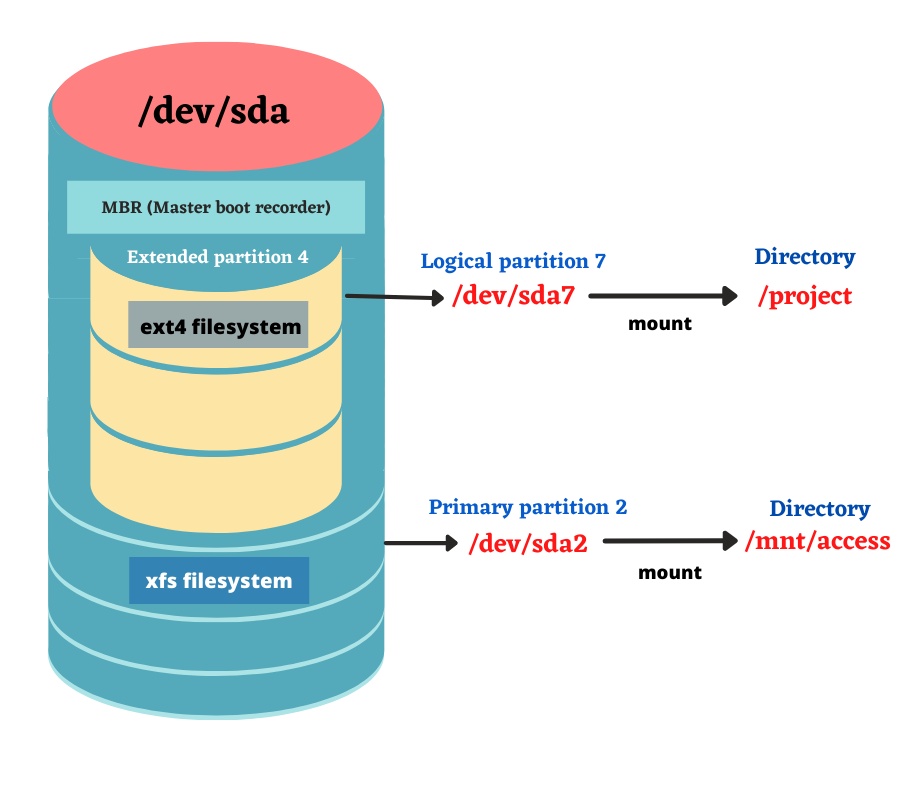
\includegraphics[scale=.6]{content/chapter8/images/new.png}
			\caption{Mounting filesystem}
			\label{mounting}
		\end{figure}	
	
	\newpage
	\paragraph{Command to mount a partition}
		\begin{itemize}		
		\item Mount a linux partition:
		\begin{tcolorbox}[breakable,notitle,boxrule=-0pt,colback=pink,colframe=pink]
			\color{black}
			\fontdimen2\font=9pt
			Syntax: mount device\_name directory\_name
			\fontdimen2\font=4pt
		\end{tcolorbox}
		
		\item Check mounted partition:
		\begin{tcolorbox}[breakable,notitle,boxrule=-0pt,colback=pink,colframe=pink]
			\color{black}
			\fontdimen2\font=9pt
			Syntax: df -Th
			\fontdimen2\font=4pt
		\end{tcolorbox}
		\bigskip
		\bigskip
		\item Eg: Create a directory to mount a partition -
		\begin{tcolorbox}[breakable,notitle,boxrule=-0pt,colback=black,colframe=black]
			\color{green}
			\fontdimen2\font=9pt
			\# mkdir /mnt/access
			\fontdimen2\font=4pt
		\end{tcolorbox}
		Mount \textbf{/dev/sda2} partition on \textbf{/mnt/access} directory -
		\begin{tcolorbox}[breakable,notitle,boxrule=-0pt,colback=black,colframe=black]
			\color{green}
			\fontdimen2\font=9pt
			\# mount /dev/sda2 /mnt/access
			\fontdimen2\font=4pt
		\end{tcolorbox}
		Check mounted partition:
		\begin{tcolorbox}[breakable,notitle,boxrule=-0pt,colback=black,colframe=black]
			\color{green}
			\fontdimen2\font=9pt
			\# df -Th
			\fontdimen2\font=4pt
		\end{tcolorbox}
		
	\end{itemize}
	\bigskip
	\begin{tcolorbox}[breakable,notitle,boxrule=1pt,colback=yellow,colframe=yellow]
		\color{black}
		Note: Mounting done using \textbf{mount} command is \textbf{temporary}. After system reboot, the partition and directory will get dissociated. This will cause partition to be \textbf{unmounted}.
	\end{tcolorbox}
	
	
	
\end{flushleft}

\newpage

